% Please keep it to 80 columns, no tabs, no trailing whitespace
% and no Windows line endings (\r\n)
\documentclass[10pt,a4paper,oneside]{report}
\usepackage{graphicx}
\usepackage{lscape}
\usepackage{float}
\usepackage{pdfpages}
\begin{document}
\title{Group 8 Integrated Project Proposal\\Project Name Here}

% Names in alphabetical order.
% The mark is for the proposal part.
\author{
  Chen Gyangyu (XX \%)\\
  Kowalczyk Mateusz (XX \%)\\
  Luff Katie (XX \%)\\
  Sampson Robert (XX \%)\\
  Singh Aman (XX \%)\\ }
%\date{}
\maketitle
\section*{Background}
Background section.

\clearpage
\subsection*{Research}
Here wa talk about what other projects like this we looked at.


\subsubsection*{Name of project we looked at 1}
Talk about the project a bit and the differences from our project.


\subsubsection*{Name of project we looked at 2}
Talk about the project a bit and the differences from our project.

\subsubsection*{Name of project we looked at 3}
Talk about the project a bit and the differences from our project.


% Screenshots from the other projects. Or something.
%% \begin{figure}[H]
%%  \caption{A screenshot of project 1} \centering
%%  \includegraphics[keepaspectratio]{project-1-placeholder.jpg}
%% \end{figure}

%% \begin{figure}[H]
%%  \caption{A screenshot of project 2} \centering
%%  \includegraphics[keepaspectratio]{project-2-placeholder.jpg}
%% \end{figure}

%% \begin{figure}[H]
%%  \caption{A screenshot of project 3} \centering
%%  \includegraphics[keepaspectratio]{project-3-placeholder.jpg}
%% \end{figure}


\clearpage
\section*{Programme and Methodology}

Aims and goals of our project. Talk about what platform it will run on
and why. Say how we're going to do research and testing. We want big
words like ``qualitative interviewing''.

\subsection*{Collaboration}
Here we talk about how we will communicate, exchange data, meeting on
time. This is where we praise version control \&c.


% We put the generated chart on the last page.
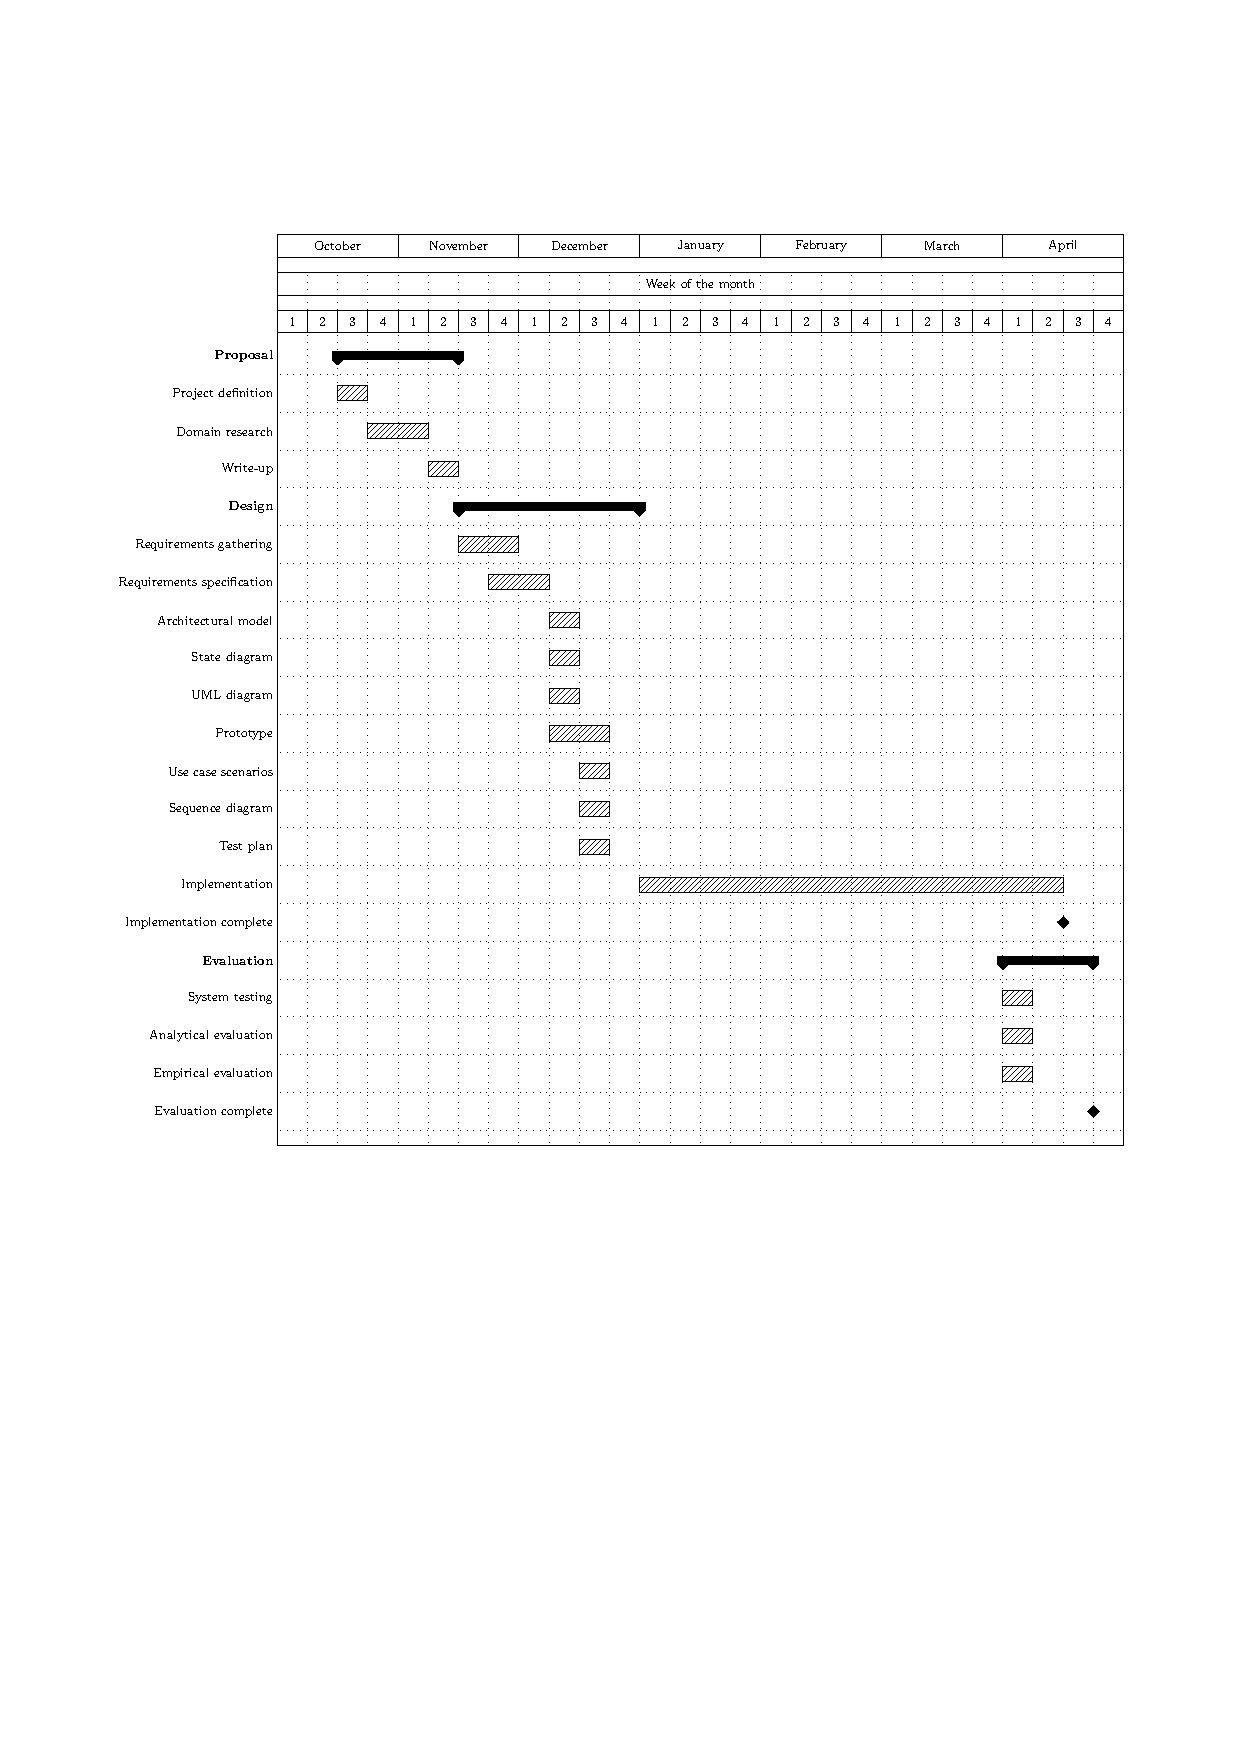
\includepdf[pages={1}]{ganttchart.pdf}

\end{document}
